\documentclass[tikz,border=5mm]{standalone}
\usetikzlibrary{calc}
\begin{document}
	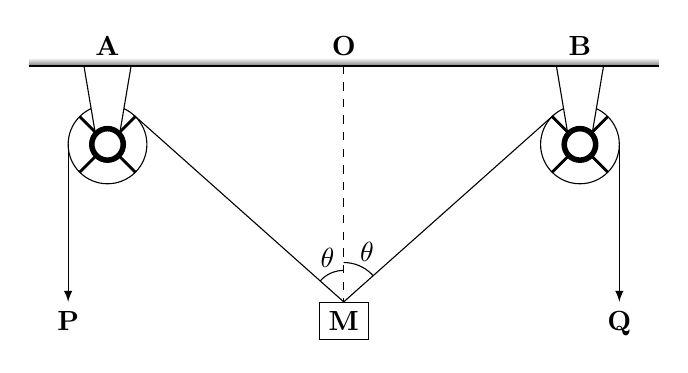
\begin{tikzpicture}
		[every node/.style={font=\bfseries}]
		\def\r{1}
		\def\a{3}
		\def\d{1}
		\path
		(0,-\a) coordinate (M) node[below,draw]{M}
		(0,0) coordinate (O) node[above]{O}
		(-\a,0) coordinate (A) node[above]{A}
		(\a,0) coordinate (B) node[above]{B}
		(-\a,-\d) coordinate (A1)--+(180:\r/2) coordinate (A2)
		(\a,-\d) coordinate (B1) --+(0:\r/2) coordinate (B2);
		% Vẽ nhánh trái
		\foreach \i in {45,135,225,-45}
		\draw[line width=1pt] (A1)--+(\i:\r/2);
		\node[circle,draw,minimum size=\r cm,outer sep=0] (cA1) at (A1){};
		\draw (M)--(tangent cs:node=cA1,point={(M)},solution=1)
		coordinate (A3);
		\draw[fill=white]
		(-\a+.3,0)--(-\a-.3,0)--($(A1)+(140:.2)$) arc(140:40:.2)--cycle;
		\draw[line width=2pt,fill=white] (A1) circle(.2);
		\draw[-latex] (A2)--+(-90:\a-\d) coordinate (P) node[below]{P};
		\begin{scope} \clip (O)--(M)--(A3);
			\draw (M) circle(4mm) node[shift={(110:6mm)}]{$\theta$};
		\end{scope}
		% Tương tự vẽ nhánh phải
		\foreach \i in {45,135,225,-45}
		\draw[line width=1pt] (B1)--+(\i:\r/2);
		\node[circle,draw,minimum size=\r cm,outer sep=0] (cB1) at (B1){};
		\draw (M)--(tangent cs:node=cB1,point={(M)},solution=2)
		coordinate (B3);
		\draw[fill=white]
		(\a+.3,0)--(\a-.3,0)--($(B1)+(140:.2)$) arc(140:40:.2)--cycle;
		\draw[line width=2pt,fill=white] (B1) circle(.2);
		\draw[-latex] (B2)--+(-90:\a-\d) coordinate (Q) node[below]{Q};
		\begin{scope} \clip (O)--(M)--(B3);
			\draw (M) circle(5mm) node[shift={(65:7mm)}]{$\theta$};
		\end{scope}
		% Trang trí phía trên
		\draw[dashed] (O)--(M);
		\shade[bottom color=black!50,top color=white]
		(-\a-1,0) rectangle (\a+1,.1);
		\draw[thick] (-\a-1,0)--(\a+1,0);
	\end{tikzpicture}
\end{document}